Floats are images, tables or other pieces of the document that are free to move to the best place in the document for them. The two most common floats are the tabular environment (for tables) and the figure environment for figures.

Use the \texttt{tabular} environment to produce basic tables. Table~\ref{tab:widgets} is produced using this code: 

\begin{lstlisting}
\begin{table}[!h]
\centering
\caption{An example table.}\label{tab:widgets}
\begin{tabular}{lr}
Item & Quantity \\
\hline
Widgets & 42 \\
Gadgets & 13
\end{tabular}
\end{table}
\end{lstlisting}

\begin{table}[!h]
\centering
\caption{An example table.}\label{tab:widgets}
\begin{tabular}{lr}
Item & Quantity \\
\hline
Widgets & 42 \\
Gadgets & 13
\end{tabular}
\end{table}

If all of the delimiters (\&) are included in each row, the table will be complete and will produce a better PDF.

To include a figure in a document, use the \texttt{figure} environment and the \texttt{includegraphics} command.

\begin{lstlisting}
\begin{figure}
\includegraphics[width=\textwidth]{figure's-file-name}
\caption{Caption goes here.}\label{fig:figuresLabel}
\end{figure}
\end{lstlisting}

Subfigures are implemented using the \texttt{subcaption} package. The example below generates Figure \ref{fig:NRELimages}.

\begin{lstlisting}
\begin{figure*}
	\centering
        \begin{subfigure}[t]{.45\linewidth}
		\centering
		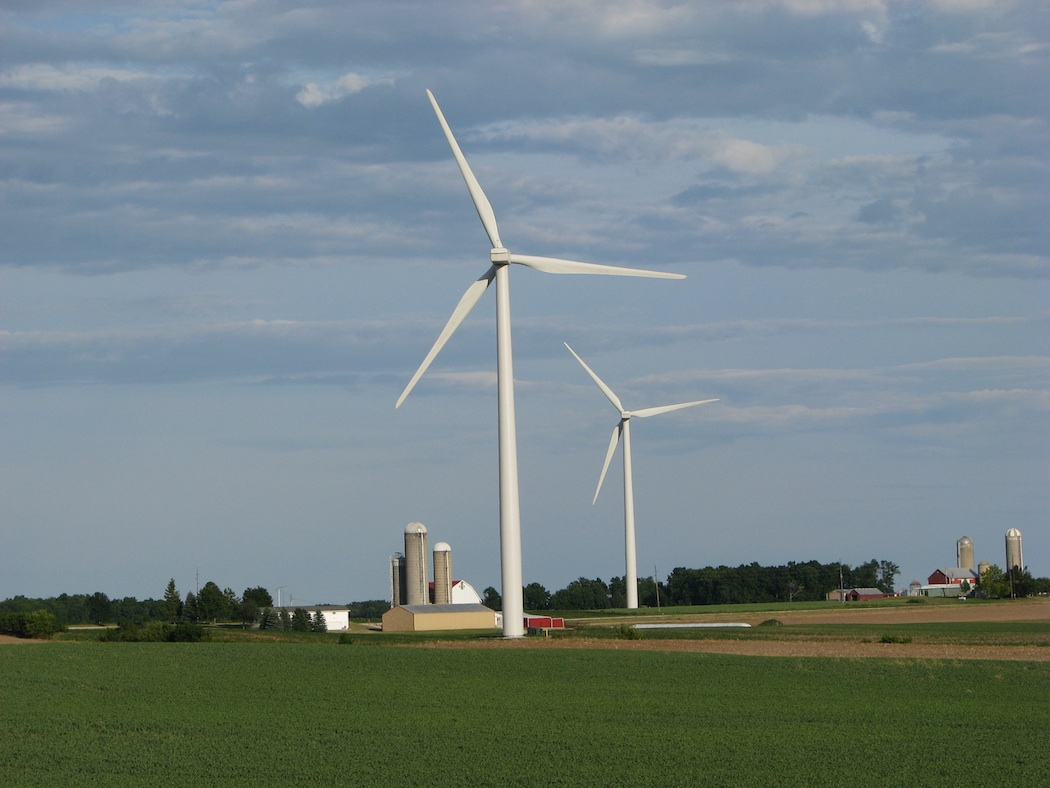
\includegraphics[height=2in]{../DemoFiles/21206}
		\caption{Wind turbines at the Forward Wind Energy Center in Fond du Lac and Dodge Counties, Wisconsin. (Photo by Ruth Baranowski / NREL)}\label{fig:21206}
	\end{subfigure}%
        \hfill
        \begin{subfigure}[t]{.45\linewidth}
		\centering
		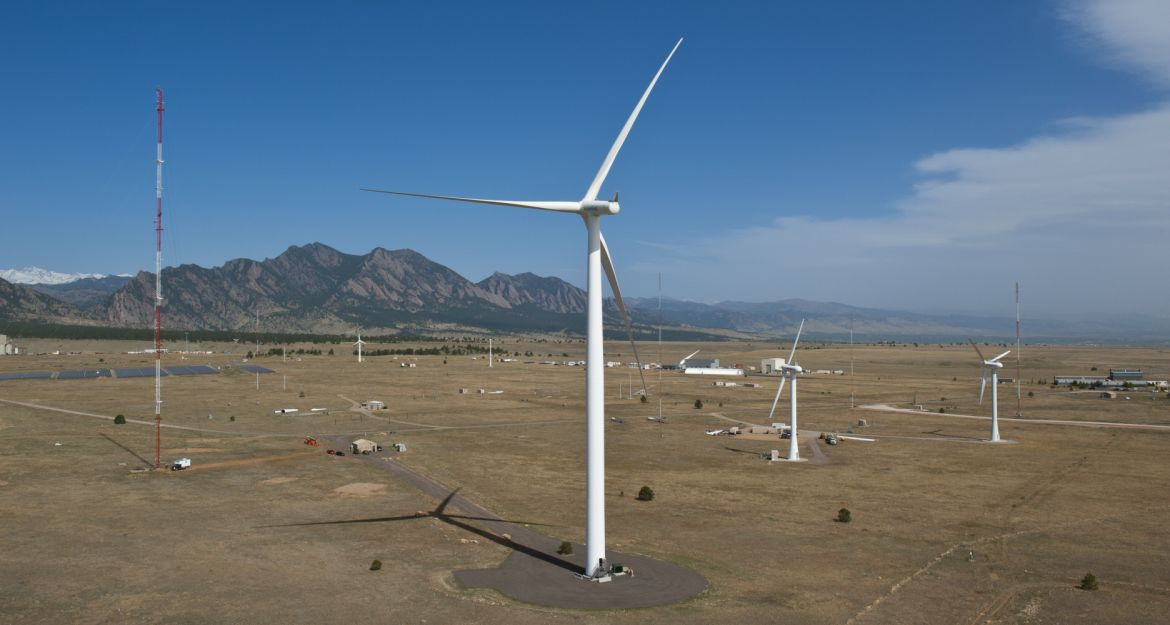
\includegraphics[height=2in]{../DemoFiles/20018}
		\caption{Aerial view of the National Wind Technology Center. (Photo by Dennis Schroeder / NREL)}\label{fig:20018}
	\end{subfigure}
	\caption{Images}\label{fig:NRELimages}
\end{figure*}
\end{lstlisting}

Note that the \texttt{subfig} and \texttt{subfigure} packages are deprecated. The \texttt{subcaption} package appears to be the most frequently maintained package at this time, and contains the same functionality as the \texttt{subfig} and \texttt{subfigure} packages.

\begin{figure*}
	\centering
        \begin{subfigure}[t]{.45\linewidth}
		\centering
		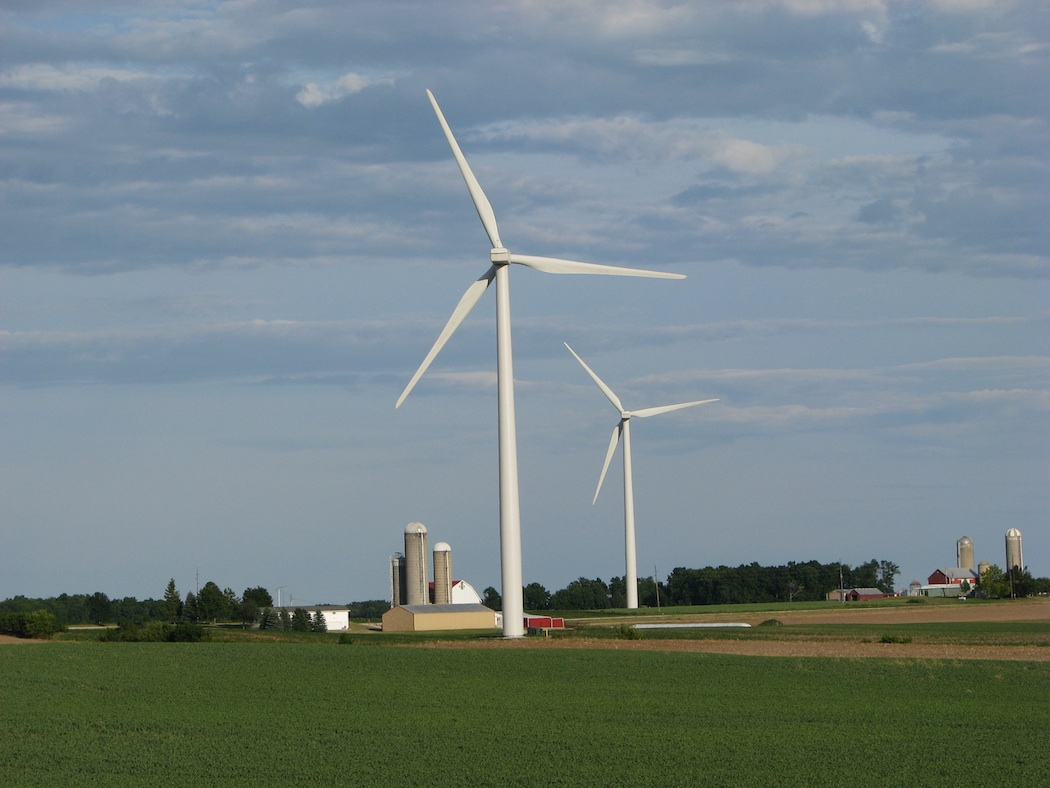
\includegraphics[height=2in]{../DemoFiles/21206}
		\caption{Wind turbines at the Forward Wind Energy Center in Fond du Lac and Dodge Counties, Wisconsin. (Photo by Ruth Baranowski / NREL)}\label{fig:21206}
	\end{subfigure}%
        \hfill
        \begin{subfigure}[t]{.45\linewidth}
		\centering
		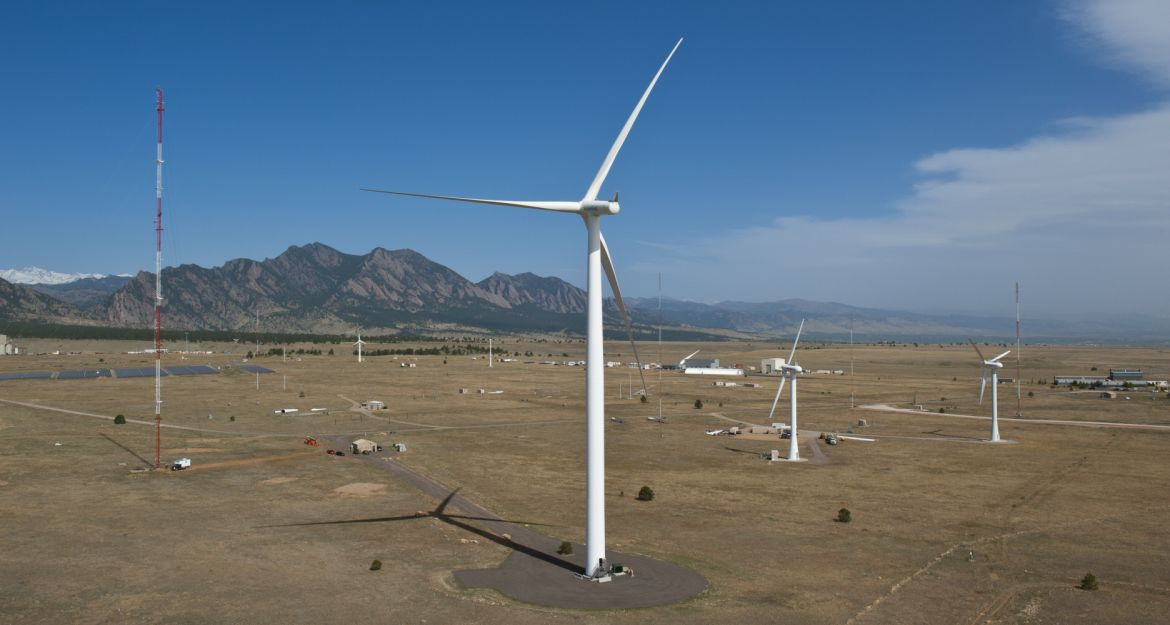
\includegraphics[height=2in]{../DemoFiles/20018}
		\caption{Aerial view of the National Wind Technology Center. (Photo by Dennis Schroeder / NREL)}\label{fig:20018}
	\end{subfigure}
	\caption{Images}\label{fig:NRELimages}
\end{figure*}
